\chapter{Analyse des besoins}


Comme on l'a vu dans l'approche théorique du \textit{Data Mining}, comme dans le cas de tout projet d'ailleurs, la définition des besoins est une étape cruciale du démarrage de l'activité. On va donc évoquer tout d'abord les besoins fonctionnels, puis les besoins non-fonctionnels.


\section{Besoins fonctionnels} 
Les besoins fonctionnels sont ceux qui permettent de remplir les conditions du cahier des charges ; ils sont incontournables. Il s'agit donc ici de voir comment on va répondre à la demande formulée à l'origine du projet.

\section{Interface utilisateur}
L'interface utilisateur se compose d'une bilibliothèque qui permettra à l'utilisateur d'exploiter les données récupérées par le parser. L'utilisateur pourra appeler les fonctions proposées par le programme ou bien écrire ses propres fonctions et les appliquer aux données.

\subsection{Se connecter à la base de données orientée documents}

\paragraph*{Description et piorité}

\textbf{Niveau de priorité = haute}

Cette bibliothèque offrira des fonctions simples d'accès en lecture/écriture sur la base de données ; de ce fait; cette librairie pourra:
\begin{itemize}
\item récupérer un \textit{Log} ou les informations générales d'un joueur
\item mettre à jour les données relatives à un \textit{Log} ou aux informations générales d'un joueur
\item créer de nouvelles données issues des analyses effectuées.
\end{itemize}

\subsection{Outils d'analyse}

\paragraph*{Description et piorité}

\textbf{Niveau de priorité = haute}

Une seconde fonctionnalité de la  bibliothèque proposera une solution à l'utilisateur pour effectuer des analyses prédéfinies sur les données récupérée, ainsi qu'un moyen d'appliquer de manière générale une analyse créée par l'utilisateur. Elle pourra donc:
\begin{itemize}
\item appliquer une fonction spécifiée par l'utilisateur à une liste de documents récupérés par une requête qu'il aura posée. La fonction spécifiée recevra un \textit{Log} et pourra travailler sur le document en question
\item générer l'ELO de chaque joueur pour chaque parti, ainsi qu'un ELO global de chaque joueur
\item détecter les différentes stratégies utilisées par les joueurs lors d'une partie ou de l'ensemble des parties
\item repérer quand le \textit{greening} survient
\end{itemize}

\iffalse
\section{Interface utilisateur}
%TODO: retravailler cette portion
L'interface utilisateur du programme sera composée d'un exécutable (\textit{dominionmining}minière de domination) qui sera exécuté avec certains paramètres pour réaliser l'action souhaitée. Le schéma ci-dessous représente les différentes interactions disponibles pour l'utilisateur:\\

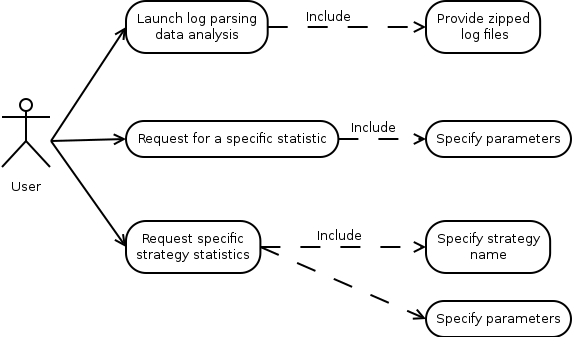
\includegraphics[scale=0.45,keepaspectratio]{diaRessources/UseCaseParsing}\\
Avant l'utilisation de toutes les fonctionnalités du programme, l'utilisateur doit lancer l'analyse.
\subsection{Lancement de l'analyse du log}
\subsubsection{Description et priorité}
\textbf{Niveau de priorité = haute}\\
\begin{itemize}
  \item L'utilisateur devra placer tous les logs compressés (fichiers tar.bz2) destinés à  être analysées dans un dossier spécifique.
  \item si aucune compression n'est donnée la compression par défaut est \textit{snappy}.
    \item Pour des fins de test, afin d'éviter d'avoir un 4 heures étape d'analyse, l'utilisateur peut spécifier un pourcentage des logs pour être analysée. en spécifiant une valeur comprise entre 0 et 100. l'analyseur choisira au hasard les logs de ceux qui sont prévus et les analyser, en créant une base de données utilisable pour des tests supplémentaires.
    \item Une fois que l'analyse est effectuée un message sera affiché sur la console (traitement de fait).

\end{itemize}

\subsection{Statistiques demandées}
\subsubsection{Description et priorité}
\textbf{Niveau de priorité = haute}\\
La demande d'une statistique peut être faite en tapant les états de \textit{dominionmining (paramètres)}.  \\
Les noms de stratégie possibles sont: big money, pen province, beyond silver.\\
Si d'autres stratégies sont reconnues par le programme, ils seront ajoutés à la liste.\\
La liste des paramètres qui seront possible d'utiliser sera déterminée dans le futur.\\

Le retour d'une statistique peut être un graphique affiché dans une fenêtre ou exportés vers un fichier. Si sa une valeur unique, un nom ou une phrase, il sera retourné à l'invite.

\subsection{Mappage des données de jeu}

Afin de permettre à l'utilisateur de demander des statistiques spécifiques concernant un jeu, le programme peut être exécuté afin de générer des logs de jeu simplifiées et un script python sera appliqué à ce log. Cela permettrait une plus grande flexibilité dans le type de statistiques affichables par le programme.
\begin{itemize}
\item Le programme sera lancé en utilisant la commande suivante: \textit{dominionmining data\_to\_query user\_script.py}
 \item Le script python sera appliquée au résultat généré et retourner les statistiques demandées par l'utilisateur.
\item Le fichier généré contenant les résultats de la requête aura le format suivant:
\begin{itemize}
\item Le nom du fichier produit est \textit{game.txt}
\item Le log simplifié contiendra chaque action effectuée par le joueur, une action par ligne. Liste des actions et leur format:
\begin{itemize}
\item Révéler une carte: \textit{joueur\_x révèle carte\_nom}
\item Piocher des cartes: \textit{joueur\_x jete n cartes}
\item Acheter une carte: \textit{joueur\_x buys carte\_name}
\item Jeter des cartes: \textit{joueur\_x trashes n cartes}
\item Mettre une carte \textit{joueur\_x puts carte\_name}
\item Gagner une carte: \textit{joueur\_x gains carte\_name}
\item Jouer une carte: \textit{joueur\_x jouer une carte\_name}

\end{itemize}
\end{itemize}
\end{itemize}
\fi



\subsection{Modélisation des données}
La première démarche consistait à modéliser les données disponibles pour créer une cohérence entre tous les formats existants. Il fallait commencer par décompresser les données, même si, comme on l'a vu, cela ne pouvait être fait que par "tranches" de temps (journées de \textit{Logs}) à cause des ressources mémoire disponibles. 

\subsubsection{Décompression des logs}
\paragraph*{Description et priorité} 



\textbf{Niveau de priorité = haute}



\begin{itemize}
  \item Les fichiers \textit{tar.bz2} seront stockés dans un dossier.
  \item Le programme va  décompresser un fichier spécifié à partir de ce dossier dans un dossier temporaire.
  \item Le programme va  supprimer les \textit{Logs} décompressés  à la demande du parser.
\end{itemize}

\subsubsection{Parser}

\paragraph*{Description et priorité} 



\textbf{Niveau de priorité = haute}



Compte tenu des problèmes mis en évidence en analysant un échantillon de \textit{Logs} (comme par exemple des incohérences de syntaxe), l'utilisation d'un parser (comme \textit{YACC} et \textit{LEX}) n'est pas recommandée. C'est pour cette raison que l'on va créer un parser qui utilisera les mots-clés et l'HTML déjà présents dans les \textit{Logs}. Ce parser sera responsable de la lecture et de la collecte des informations importantes sans perdre la structure du \textit{Log}.
Un aperçu des données devant être reconnues par le parser est représenté dans l'illustration suivante :\\


\includegraphics[scale=0.35,keepaspectratio]{diaRessources/UseCaseParser}

\begin{itemize}
\item Winners: liste des gagnants du jeu ; il peut y avoir plusieurs gagnants en cas d'égalité.
\item Market: liste des 10 cartes disponibles pour être achetées par les joueurs.
\item Cards Gone: liste des cartes qui ont été entièrement acquises à la fin de la partie.
\item First hand: liste des cartes obtenues au début de la partie.%à voir
\item Player Name: nom du joueur.
\item Victory points: nombre de points à la fin de la partie.
\item Player cards: liste des cartes obtenues à la fin de jeu avec des noms et de quantités differents.
\item Victory cards: liste des cartes de victoire le joueur avec le acheté.
\item Trash: liste des cartes qui sont jetés à la fin de la partie.
\item Game Moves: liste des actions effectuées pendant chaque tour d'un joueur.
\end{itemize}
Lorsque l'utilisateur exécute le parser, celui-ci va identifier les types d'informations concernant chacun des éléments représentés dans le graphique précédent, les trier, et les charger dans une structure de données du type "document", puis alimenter la base de données avec le document. \\

\subsubsection{Créer le game-log}
\paragraph*{Description et priorité}
\textbf{Niveau de priorité = haute}\\
Cette fonctionnalité consiste à créer une structure de données dans laquelle les données du \textit{Log} seront chargées.
La figure suivante est la représentation graphique d'une vue d'ensemble de la structure des données:\\
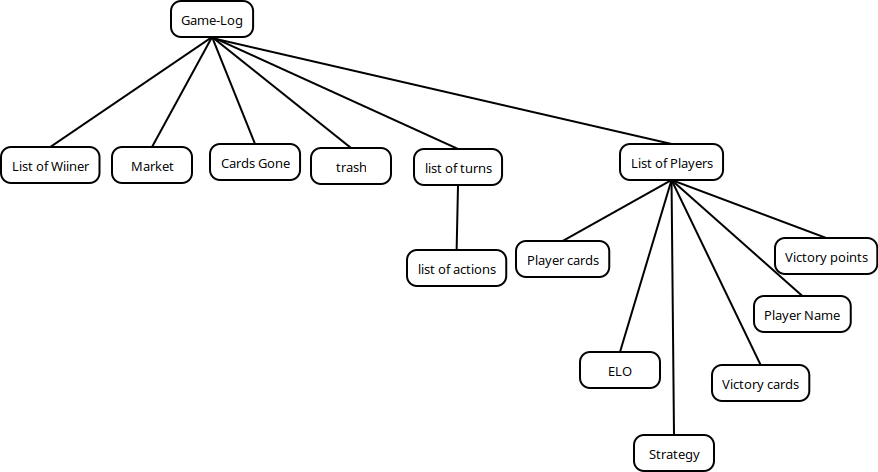
\includegraphics[scale=0.5,keepaspectratio]{diaRessources/game-log}

\subsubsection{Créer une base de données orientée document }

\paragraph*{Description et priorité}
\textbf{Niveau de priorité = haute}\\
Ce module sera responsable de la création de la base de données orientée document, contenant des données au format JSON.
\subsubsection{Se connecter à la base de données orientée document }
\paragraph*{Description et priorité}
\textbf{Niveau de priorité = haute}\\
 Un interface complet de communication avec la base de données orientée document permettra d'envoyer et recevoir des données.


\subsubsection{Compression}
\paragraph*{Description et priorité}
\textbf{Niveau de priorité = moyen}\\

La base de données orientée document contiendra la totalité des données et un certain niveau de compression devra être appliqué.
La base de données que nous allons utiliser est \textit{mongoDB}, et elle offre 2 niveaux de compression \textit{Zlib} et \textit{Snappy}.
Au cours du développement, on utilise \textit{Snappy}, car il offre une meilleure performance.
Mais le programme final devrait donner à l'utilisateur la possibilité de choisir le niveau de compression lors du démarrage de l'analyse du \textit{Log}.

\subsubsection{Sauvegarder le game-log}

\paragraph*{Description et priorité}
\textbf{Niveau de priorité = haute}\\

Cette fonctionnalité permet d'envoyer les documents au format JSON et de les stocker dans la base de données. 

%partie de python à discuter


\subsubsection{Restorer le \textit{game-log}}
\paragraph*{Description et priorité}
\textbf{Niveau de priorité = moyen}\\

Cette fonction a pour responsabilité de restaurer l'information manquante sur les \textit{Logs} analysés, par déduction, sur la base des informations déjà récoltées dans le \textit{Log}. Si les échanges exécutés pendant la partie sont fournis par le \textit{Log} on va les utiliser pour simuler la partie et reconstituer les éléments manquants. \\

En cas d'un en-tête du jeu manquant par exemple, on utilisera la stratégie suivante :
  \begin{itemize}
\item \textit{Gagnants / "cartes bonus" / points "bonus" manquants }: le programme peut garder la trace des cartes détenues par les joueurs pendant le jeu afin de savoir combien de "cartes bonus" ils ont à la fin de la partie.
\item \textit\textit{{Market} manquant}: le programme peut garder la trace des cartes achetées au cours du jeu afin de reconstituer partiellement ou totalement les cartes disponibles sur \textit{Market}.
\item \textit{Cartes \textit{Gone}}: comme avec les données de \textit{Market} manquantes, le programme permet de garder une trace des cartes achetées et compter la quantité achetée pour chaque carte ; si le montant maximum de cartes est acheté, la carte a disparu à la fin de la partie.
\item \textit{Nom du joueur manquant}: le jeu signale à chaque mouvement le nom du joueur qui agit. Le programme sera donc tout simplement chargé de les restaurer dans l'en-tête.
\item \textit{Cartes de joueur}: le programme garde une trace des actions effectuées au cours du jeu en ce qui concerne les cartes de joueurs (actions, tirage,...) et d'en garder la liste.
  \end{itemize}


\subsubsection{Plotting}
\paragraph*{Description et priorité}
\textbf{Niveau de priorité = haute}\\

La bibliothèque devra comporter une fonctionnalité de \textit{plotting} qui permet de visualiser  les données converties obtenues.
\subsubsection{Calculer l'\textit{\textbf{ELO}}}
%TODO
\paragraph*{Description et priorité}
\textbf{Niveau de priorité = haute}\\

L'analyseur devra calculer l'ELO final de chaque joueur ainsi que son ELO temporaire à l'issue de chaque partie.\newline
Pour chaque partie; dans l'ordre chronologique, l'analyseur va calculer l'ELO de chaque joueur à l'issue de cette partie et l'ajouter aux données relatives au \textit{Log} en question ; il va également mettre à jour l'ELO général des joueurs concernés afin de pouvoir continuer à calculer leur évolution.


\iffalse
%TODO: refaire le diagramme du calcul de l'elo
Le schéma suivant illustre le processus du calcul de ELO :\\
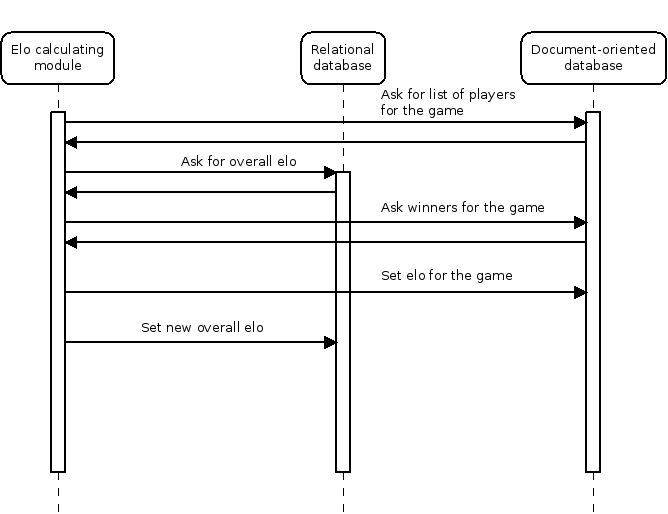
\includegraphics[width=\textwidth,height=\textheight,keepaspectratio]{diaRessources/elocalc}\\
\fi
\subsubsection{Reconnaître les stratégies}
\paragraph*{Description et priorité}
\textbf{Niveau de priorité = moyen}\\

Le wiki de dominion décrit quelques stratégies qui peuvent être utilisés dans le jeu.\\Par exemple :\\
\textit{Big Money}\\
\textit{Beyond Silver}\\
\textit{Penultimate Province Rule}\\
L'intérêt du présent projet, comme on l'a vu, est de vérifier la validité des stratégies conseillées par le wiki. Celles qui seraient déduites par le projet seraient fondeées sur un calcul approfondi dépassant les simples intuitions ou calculs statistiques concernant ces mêmes stratégies. Mais cette méthode, pour efficace qu'elle soit, est bien entendu beaucoup plus coûteuse en temps et en efforts.
\\

\textbf{Cette image décrit le processus de décision associé à la stratégie Big Money}\\
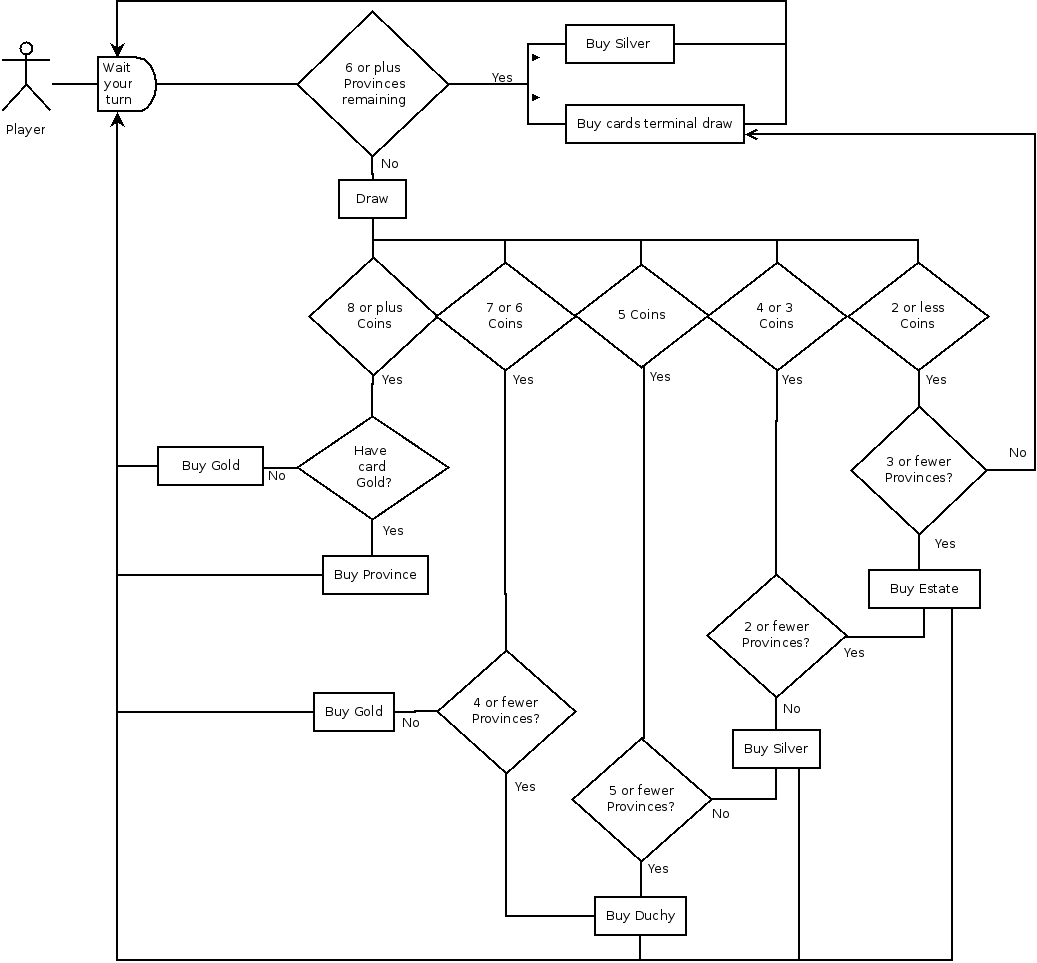
\includegraphics[width=\textwidth,height=\textheight,keepaspectratio]{diaRessources/big-money}\\
%The analyzer has to recognize when a player buys only money cards and specific cards related to the big money strategy. It also has to keep track of the remaining provinces to be bought.\\
L'analyseur devra donc être en mesure de reconnaître quelle stratégie a été utilisée sur un match donné (si une  stratégie a été utilisée), et d'attribuer à chaque partie le nom de la stratégie utilisée par chaque joueur, puis d'enregistrer le tout sur la base de données.\\


Afin de reconnaître la stratégie \textit{Beyond Silve}r ou \textit{Big Money}, l'analyseur doit reconnaître lorsque certains types de cartes sont achetées (la liste de ces cartes peut être trouvée sur : \url{http://wiki.dominionstrategy.com/index.php/Silver#Beyond_Silver} et \url{http://wiki.dominionstrategy.com/index.php/Big_Money})\\

Afin de reconnaître que \textit{Penultimate Province Rule} a été utilisée, (comme expliqué à \url{http://dominionstrategy.com/2011/03/28/the-penultimate-province-rule/}), l’analyseur doit garder une trace de la quantité de "Cartes bonus" de chaque joueur à chaque tour.

\subsubsection{Reconnaître le \textit{Greening}}
\paragraph*{Description et priorité}
\textbf{Niveau de priorité = haute}\\

L'analyseur doit être capable de reconnaître à quel moment les joueures commencent à investir dans les "Cartes bonus", et donc à pratiquer le \textit{\textbf{greening}} dans chaque match.
En savoir plus à propos de \textit{\textbf{greening}} sur \url{http://wiki.dominionstrategy.com/index.php/Greening}.\\ 

\newpage

\section{Besoins non-fonctionnels}
Les besoins non-fonctionnels sont des possibilités qui n'ont pas été expressément réclamées par le client, et donc n'appartiennent pas au cahier des charges. Néanmoins, si on peut les mettre en oeuvre, elles constituent un plus appréciable et augmentent la dimension qualitative du travail.

\subsection{Besoins de performance}

Aucun besoin de performance spécifique n’a été exprimé par le client. Cependant, il tombe sous le sens qu'il convient d'optimiser l'exécution des différentes tâches en termes de rapidité et d'accessibilité pour l'utilisateur.\\


\subsection{Fiabilité}
Le client demande qu'un maximum de \textit{Logs} soient récupérés, la totalité des \textit{Logs} ne pourra pas être parsée mais une tolérance de 5 à 10\% de \textit{Logs} peut être acceptée.\newline
En revanche lorsque un \textit{Log} est parsé, le programme devra récuperer 100\% des données présentes le concernant, et si possible restaurer les informations non présentes dans le \textit{Log} de départ.

\subsection{Attributs de qualité de logiciels}

Le programme devra pouvoir lancer la phase initiale de parsing en une seule ligne de commande.\\
Les fonctions présentes dans la librairie à l'attention de l'utilisateur devront avoir un nom clair et facile à comprendre.\\
Les données générées par l'analyseur n’ont pas besoin à être lisibles par l'homme.\\
Les game log générés devront pouvoir être analysés par l'utilisateur afin de permettre la plus grande souplesse possible dans le traitement des logs.

\section{Besoins organisationnels}

La répartition des tâches du projet et l'estimation de la durée de chacune d'elle sont présentées sur le planning suivant:\\

\subsection{Planning prévisionnel}

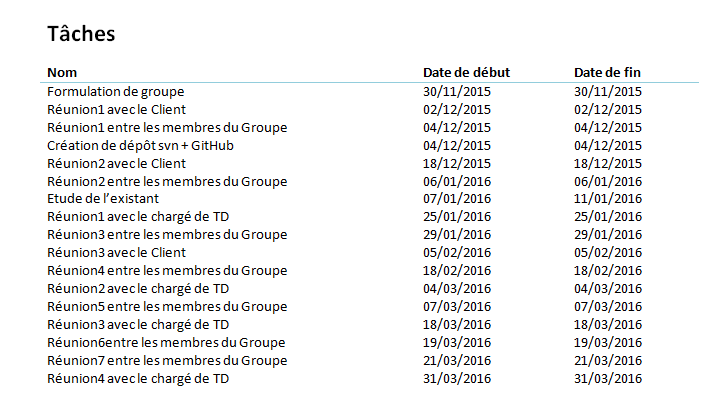
\includegraphics[scale=0.45,keepaspectratio]{planning}\\

\subsection{Diagramme de Gantt}

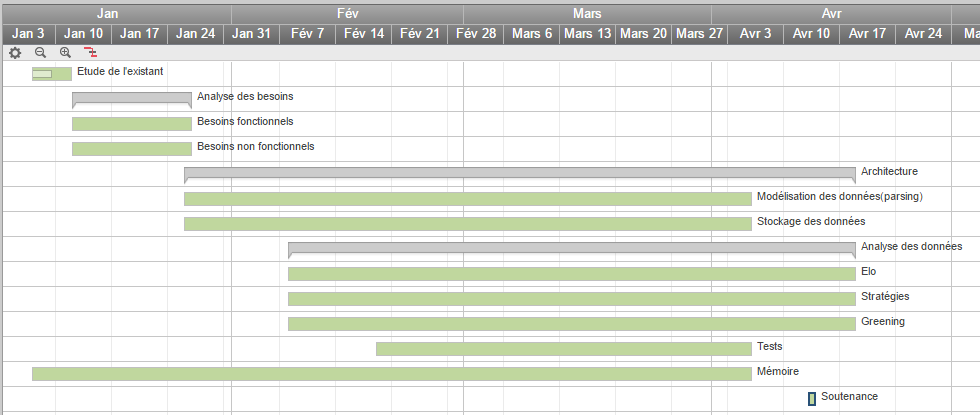
\includegraphics[scale=0.45,keepaspectratio]{gantt}\\

\newpage
\iffalse
\section{Développement}

Intro

\subsection{Tâches}

Bla\\


%tableau à taille fixée sur certaines colonnes (param sur la ligne \begin{tabularx}, voir wiki pour plus d'info sur la syntaxe
\begin{figure}[!h]
\begin{center}
\begin{tabularx}{17cm}{|c|p{6cm}|X|}
  \hline
  Priorité & Nom & Raison\\
  \hline
  1 & Tache 1 & Doit être vérifié en premier car sinon [...] \tabularnewline
  2 & Tache 2 & On doit pouvoir [...] \tabularnewline
  3 & Tache 3 & Comme les principales fonctionnalités permettant de tester sont opérationnelles, nous pouvons passer à cette tâche. \tabularnewline
  4 & Tache 4 & Parce que [...] \tabularnewline
  5 & Tache 5 & La tache 5 fait partie des principales [...]. \tabularnewline
  6 & Tache 6 & Dernière fonctionnalité essentielle à mettre en place. \tabularnewline
  7 & Tache 7 & Non-essentiel, mais apporterait un plus au projet. \tabularnewline
  8 & Tache 8 & Non-essentiel, mais apporterait un plus au projet. \tabularnewline
  \hline
\end{tabularx}
\end{center}
\caption{Tableau récapitulatif des tâches}
\end{figure}

\subsection{Tests}

Bla\\

\begin{figure}[!h]
\begin{center}
\begin{tabularx}{17cm}{|p{6cm}|X|}
  \hline
  Fonctionnalité & Test\\
  \hline
  Fonction 1 & Quand [...], vérifier [...]. \tabularnewline
  & Et quand [...], vérifier [...]. \tabularnewline
  Fonction 2 & Vérifier [...]. \tabularnewline
  Fonction 3 & Vérifier [...]. \tabularnewline
  Fonction 4 & Avoir [...]. \tabularnewline
  Fonction 5 & Accéder à [...]. \tabularnewline
   & Vérifier que [...]. \tabularnewline
  Fonction 6 & Accéder à [...]. \tabularnewline
   & Et vérifier [...]. \tabularnewline
  Fonction 7 & Installer [...]. \tabularnewline
   & Vérifier [...]. \tabularnewline
  Fonction 8 & Compter [...]. \tabularnewline
  \hline
\end{tabularx}
\end{center}
\caption{Tableau récapitulatif des tests}
\end{figure}
\fi
